\documentclass{beamer}
\usepackage[utf8]{inputenc}

\usetheme{Madrid}
\usecolortheme{default}
\usepackage{amsmath,amssymb,amsfonts,amsthm}
\usepackage{txfonts}
\usepackage{tkz-euclide}
\usepackage{listings}
\usepackage{adjustbox}
\usepackage{array}
\usepackage{tabularx}
\usepackage{gvv}
\usepackage{lmodern}
\usepackage{circuitikz}
\usepackage{tikz}
\usepackage{graphicx}
 \graphicspath{{figs/}}
\setbeamertemplate{page number in head/foot}[totalframenumber]
\usepackage[T1]{fontenc}
\usepackage{lmodern}

\usepackage{tcolorbox}
\tcbuselibrary{minted,breakable,xparse,skins}

\definecolor{bg}{gray}{0.95}
\DeclareTCBListing{mintedbox}{O{}m!O{}}{%
  breakable=true,
  listing engine=minted,
  listing only,
  minted language=#2,
  minted style=default,
  minted options={%
    linenos,
    gobble=0,
    breaklines=true,
    breakafter=,,
    fontsize=\small,
    numbersep=8pt,
    #1},
  boxsep=0pt,
  left skip=0pt,
  right skip=0pt,
  left=25pt,
  right=0pt,
  top=3pt,
  bottom=3pt,
  arc=5pt,
  leftrule=0pt,
  rightrule=0pt,
  bottomrule=2pt,
  toprule=2pt,
  colback=bg,
  colframe=orange!70,
  enhanced,
  overlay={%
    \begin{tcbclipinterior}
    \fill[orange!20!white] (frame.south west) rectangle ([xshift=20pt]frame.north west);
    \end{tcbclipinterior}},
  #3,
}

\lstset{
    language=C,
    basicstyle=\ttfamily\small,
    keywordstyle=\color{blue},
    stringstyle=\color{orange},
    commentstyle=\color{green!60!black},
    numbers=left,
    numberstyle=\tiny\color{gray},
    breaklines=true,
    showstringspaces=false,
}

% ------- Macros matching your style -------
\renewcommand{\vec}[1]{\mathbf{#1}}

% ------- Title (mirrors your current problem) -------
\title{4.3.10}
\author{Aniket-EE25BTECH11007}

\begin{document}
\frame{\titlepage}

% ===================== QUESTION =====================
\begin{frame}{Question}
Find the direction and normal vectors of the line \(x - y = 2\).
\end{frame}

% ===================== THEORETICAL SOLN (1) =====================
\begin{frame}{Theoretical Solution}
\begin{equation}
\begin{pmatrix} x \\ y \end{pmatrix}
=
\begin{pmatrix} 0 \\ c \end{pmatrix}
+ x
\begin{pmatrix} 1 \\ m \end{pmatrix}
\label{eq:param}
\end{equation}
where $\begin{pmatrix} 1 \\ m \end{pmatrix}$ is the direction vector and $m$ is the slope.

\begin{equation}
\vec{n}^{\top}\,x = c
\label{eq:normal}
\end{equation}
where $\vec{n}$ is the normal vector of the line.

\begin{equation}
\vec{n}^{\top}
\begin{pmatrix} 1 \\ m \end{pmatrix}
= 0
\label{eq:orth}
\end{equation}

From $x - y = 2$ ,the slope is $m=1$. Hence, using \eqref{eq:param},
\begin{equation}
\begin{pmatrix} x \\ y \end{pmatrix}
=
\begin{pmatrix} 0 \\ -2 \end{pmatrix}
+ x
\begin{pmatrix} 1 \\ 1 \end{pmatrix}
\label{eq:param-inst}
\end{equation}
\end{frame}

% ===================== THEORETICAL SOLN (2) =====================
\begin{frame}{Theoretical Solution}
Let $\begin{pmatrix} x \\ y \end{pmatrix}$ be a normal vector. Then, from \eqref{eq:orth},
\begin{equation}
\begin{pmatrix} x \\ y \end{pmatrix}^{\!\top}
\begin{pmatrix} 1 \\ 1 \end{pmatrix}
= 0
\quad\Longrightarrow\quad
x + y = 0
\quad\Longrightarrow\quad
\begin{pmatrix} x \\ y \end{pmatrix}
=
\begin{pmatrix} 1 \\ -1 \end{pmatrix}
\label{eq:normal-inst}
\end{equation}

Line in normal form using \eqref{eq:normal} 
\[
\begin{pmatrix} 1 \\ -1 \end{pmatrix}^{\!\top}
\begin{pmatrix} x \\ y \end{pmatrix}
= 2
\]


Hence, the direction vector is
$\displaystyle \begin{pmatrix} 1 \\ 1 \end{pmatrix}$,
and the normal vector is
$\displaystyle \begin{pmatrix} 1 \\ -1 \end{pmatrix}$.

\end{frame}

% ===================== C CODE (1) =====================
\begin{frame}[fragile]{C Code}
\begin{lstlisting}
// mg4.c
#include <math.h>

double arr_dot(const double *u, const double *v, int n) {
    double sum = 0.0;
    for (int i = 0; i < n; ++i) sum += u[i] * v[i];
    return sum;
}

double arr_norm(const double *u, int n) {
    double s = arr_dot(u, u, n);
    if (s <= 0.0) return 0.0;
    return sqrt(s);
}

void arr_scale(const double *u, double k, double *out, int n) {
    for (int i = 0; i < n; ++i) out[i] = k * u[i];
}
\end{lstlisting}
\end{frame}

% ===================== C CODE (2) =====================
\begin{frame}[fragile]{C Code}
\begin{lstlisting}
void arr_normalize(const double *u, double *out, int n) {
    double r = arr_norm(u, n);
    if (r == 0.0) {
        for (int i = 0; i < n; ++i) out[i] = 0.0;
    } else {
        for (int i = 0; i < n; ++i) out[i] = u[i] / r;
    }
}

/* Line: ax + by = c
   normal    = (a, b)
   direction = (-b, a)  (perpendicular to normal)
*/
void line_direction_normal(double a, double b, double c,
                           double *dir_out,      /* len 2 */
                           double *normal_out) { /* len 2 */
    (void)c;               /* c not needed for vectors */
    normal_out[0] = a;     normal_out[1] = b;
    dir_out[0]    = -b;    dir_out[1]    = a;
}
\end{lstlisting}
\end{frame}

% ===================== PY + C (1) =====================
\begin{frame}[fragile]{Python + C}
\begin{lstlisting}
import ctypes
from ctypes import c_double, c_int, POINTER
import numpy as np
import matplotlib.pyplot as plt

lib = ctypes.CDLL("./mg4.so")

lib.arr_dot.argtypes  = [POINTER(c_double), POINTER(c_double), c_int]
lib.arr_dot.restype   = c_double
lib.arr_norm.argtypes = [POINTER(c_double), c_int]
lib.arr_norm.restype  = c_double
lib.arr_normalize.argtypes = [POINTER(c_double), POINTER(c_double), c_int]
lib.arr_normalize.restype  = None
lib.line_direction_normal.argtypes = [c_double, c_double, c_double,
                                      POINTER(c_double), POINTER(c_double)]
lib.line_direction_normal.restype  = None
\end{lstlisting}
\end{frame}

% ===================== PY + C (2) =====================
\begin{frame}[fragile]{Python + C }
\begin{lstlisting}
def cvec(arr):
    arr = np.asarray(arr, dtype=float)
    return (c_double * arr.size)(*arr.tolist()), arr.size

def dot(u, v):
    cu, n = cvec(u); cv, _ = cvec(v)
    return lib.arr_dot(cu, cv, n)

def normalize(u):
    cu, n = cvec(u)
    out = (c_double * n)()
    lib.arr_normalize(cu, out, n)
    return np.array([out[i] for i in range(n)], dtype=float)

# Solve x - y = 2  (a=1, b=-1, c=2)
a, b, c = 1.0, -1.0, 2.0
d = (c_double * 2)()
n = (c_double * 2)()
lib.line_direction_normal(a, b, c, d, n)

d_np = np.array([d[0], d[1]])
n_np = np.array([n[0], n[1]])
ud = normalize(d_np)
un = normalize(n_np)
\end{lstlisting}
\end{frame}

% ===================== PY + C (3) =====================
\begin{frame}[fragile]{Python + C }
\begin{lstlisting}
print("Direction (raw):", d_np.tolist())   # [1.0, 1.0]
print("Normal   (raw):", n_np.tolist())    # [1.0, -1.0]
print("dot(direction, normal) =", dot(d_np, n_np))

x = np.linspace(-2, 6, 200)
y = x - 2

x0, y0 = 2.0, 0.0
scale = 2.0

plt.figure()
plt.plot(x, y, label="x - y = 2")
plt.quiver([x0], [y0], [ud[0]*scale], [ud[1]*scale],
           angles='xy', scale_units='xy', scale=1, label="direction")
plt.quiver([x0], [y0], [un[0]*scale], [un[1]*scale],
           angles='xy', scale_units='xy', scale=1, label="normal")
plt.gca().set_aspect('equal', adjustable='box')
plt.xlabel("x"); plt.ylabel("y")
plt.title("Line x - y = 2 with direction and normal vectors")
plt.grid(True); plt.legend(); plt.show()
\end{lstlisting}
\end{frame}

% ===================== PURE NUMPY (1) =====================
\begin{frame}[fragile]{Python}
\begin{lstlisting}
import numpy as np
import matplotlib.pyplot as plt

def dot(u, v):
    u = np.asarray(u, dtype=float)
    v = np.asarray(v, dtype=float)
    if u.shape != v.shape:
        raise ValueError("dot: shapes must match")
    return float(np.dot(u, v))

def norm(u):
    u = np.asarray(u, dtype=float)
    return float(np.sqrt(np.dot(u, u)))

def normalize(u):
    u = np.asarray(u, dtype=float)
    r = norm(u)
    return u / r if r != 0.0 else np.zeros_like(u)
\end{lstlisting}
\end{frame}

% ===================== PURE NUMPY (2) =====================
\begin{frame}[fragile]{Python}
\begin{lstlisting}
def line_direction_normal(a, b, c):
    d = np.array([-b, a], dtype=float)  # direction
    n = np.array([a,  b], dtype=float)  # normal
    return d, n

a, b, c = 1.0, -1.0, 2.0
d, n = line_direction_normal(a, b, c)
ud, un = normalize(d), normalize(n)

print("Direction (raw):", d.tolist())        # [1.0, 1.0]
print("Normal   (raw):", n.tolist())         # [1.0, -1.0]
print("dot(direction, normal) =", dot(d, n)) # 0.0

x = np.linspace(-2, 6, 200)
y = x - 2
x0, y0 = 2.0, 0.0
scale = 2.0

plt.figure()
plt.plot(x, y, label="x - y = 2")
plt.quiver([x0], [y0], [ud[0]*scale], [ud[1]*scale],
           angles='xy', scale_units='xy', scale=1, label="direction")
plt.quiver([x0], [y0], [un[0]*scale], [un[1]*scale],
           angles='xy', scale_units='xy', scale=1, label="normal")
plt.gca().set_aspect('equal', adjustable='box')
plt.xlabel("x"); plt.ylabel("y")
plt.title("NumPy: line x - y = 2 with direction and normal")
plt.grid(True); plt.legend(); plt.show()
\end{lstlisting}
\end{frame}

% ===================== PLOT SLIDE =====================
\begin{frame}{Plot}
    \centering
    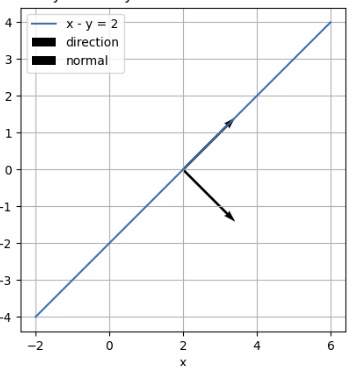
\includegraphics[width=\columnwidth, height=0.8\textheight, keepaspectratio]{figs/mg4plot.png}
\end{frame}

\end{document}
